\documentclass[a4paper,12pt]{article}
\usepackage{times}
\usepackage[francais]{babel}
\usepackage[utf8x]{inputenc}
\usepackage[T1]{fontenc}
\usepackage{amsmath}
\usepackage{amssymb}
\usepackage{graphicx}
\usepackage{pdfpages}
\usepackage{pdflscape}
\usepackage{listings}
\usepackage{longtable}
\lstset{literate=
{é}{{\'e}}1
{è}{{\`e}}1
{ê}{{\^e}}1
{à}{{\`a}}1
{â}{{\^a}}1
}
\lstset{language=C++,
                basicstyle=\footnotesize,
                keywordstyle=\footnotesize\color{blue},
                otherkeywords={override,nullptr}
}
\definecolor{orange}{rgb}{0.8,0.4,0.0}
\definecolor{darkblue}{rgb}{0.0,0.0,0.6}
\definecolor{cyan}{rgb}{0.0,0.6,0.6}
\lstdefinelanguage{JSON}
{
  basicstyle=\normalsize,
  columns=fullflexible,
  showstringspaces=false,
  commentstyle=\color{gray}\upshape,
  morestring=[b]",
  morestring=[s]{>}{<},
  morecomment=[s]{<?}{?>},
  stringstyle=\color{orange},
  identifierstyle=\color{darkblue},
  keywordstyle=\color{blue},
  morekeywords={string,number,array,object}% list your attributes here
}

\sloppy

\setlength{\topmargin}{0cm}
\setlength{\headsep}{0.in}
\setlength{\headheight}{0.in}
\setlength{\evensidemargin}{0cm}
\setlength{\oddsidemargin}{-1cm}
\textwidth 18cm
\textheight 25cm

\begin{document}

\thispagestyle{empty}

\begin{titlepage}

\vspace*{2cm}

\begin{center}\textbf{\Huge Projet Logiciel Transversal}\end{center}{\Large \par}

\begin{center}\textbf{\large Auteurs}\end{center}{\large \par}

\vspace{2cm}

%\begin{figure}[h]
%\begin{center}
%\includegraphics[width=\textwidth]{exemple.png}
%\caption{\label{pacmangame}Exemple du jeu}
%\end{center}
%\end{figure}

\clearpage

{\small
\tableofcontents
}

\end{titlepage}

\clearpage
\section{Présentation Générale}

\subsection{Archétype}


\subsection{Règles du jeu}

\subsection{Ressources}



\clearpage
\section{Description et conception des états}

\subsection{Description des états}


\subsection{Conception Logiciel}


%\begin{landscape}
%\begin{figure}[p]
%\includegraphics[width=0.9\paperheight]{state.pdf}
%\caption{\label{uml:state}Diagramme des classes d'état.} 
%\end{figure}
%\end{landscape}

\clearpage
\section{Rendu: Stratégie et Conception}

\subsection{Stratégie de rendu d'un état}


\subsection{Conception logiciel}

%\begin{landscape}
%\begin{figure}[p]
%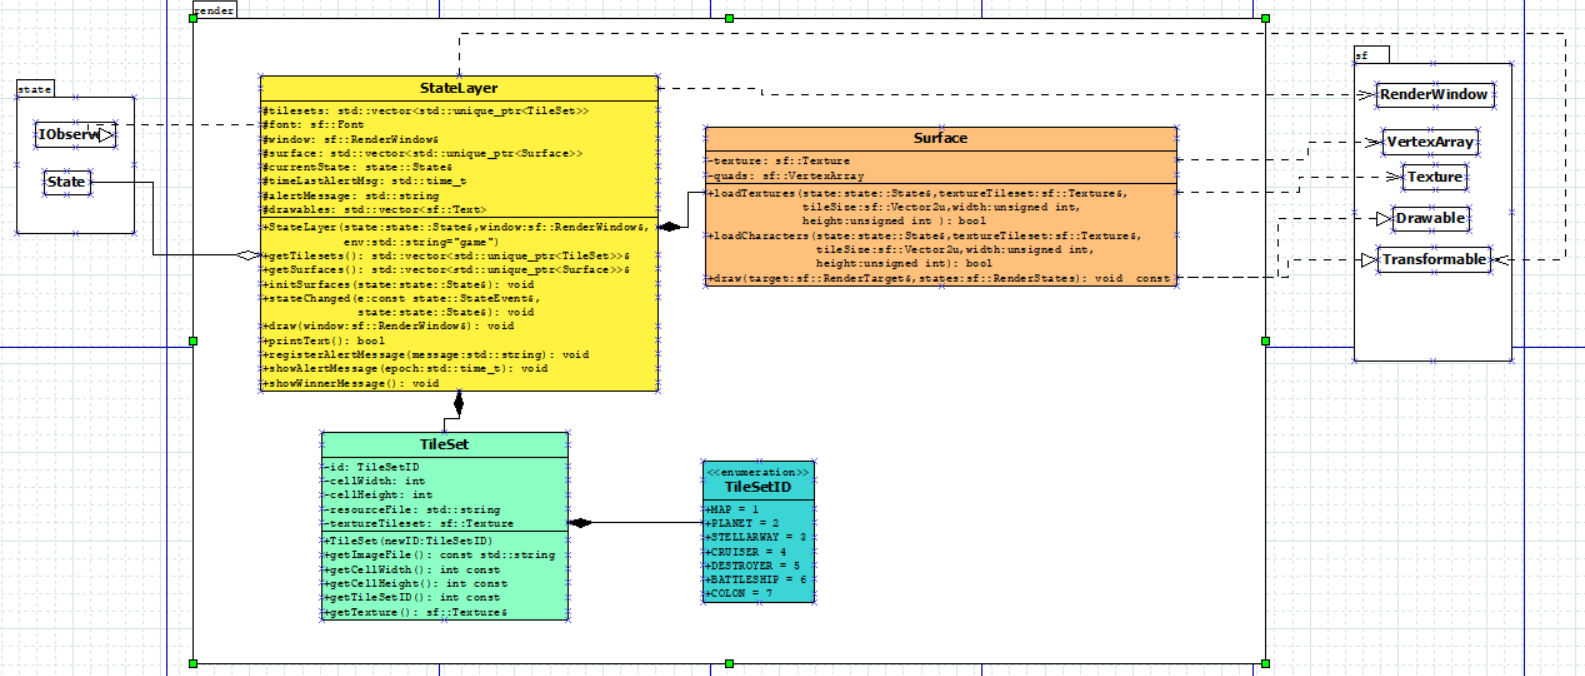
\includegraphics[width=0.9\paperheight]{render.pdf}
%\caption{\label{uml:render}Diagramme des classes de rendu.} 
%\end{figure}
%\end{landscape}

\clearpage
\section{Règles de changement d'états et moteur de jeu}

\subsection{Règles}

\clearpage
\subsection{Conception logiciel}


%\begin{landscape}
%\begin{figure}[p]
%\includegraphics[width=0.9\paperheight]{engine.pdf}
%\caption{\label{uml:engine}Diagramme des classes de moteur de jeu.} 
%\end{figure}
%\end{landscape}


\section{Intelligence Artificielle}

\subsection{Stratégies}

\clearpage
\subsection{Conception logiciel}


%\begin{landscape}
%\begin{figure}[p]
%\includegraphics[width=0.9\paperheight]{ai.pdf}
%\caption{\label{uml:ai}Diagramme des classes d'intelligence artificielle.} 
%\end{figure}
%\end{landscape}


\section{Modularisation}
\label{sec:module}

\subsection{Organisation des modules}

\clearpage
\subsection{Conception logiciel}


%
%\begin{landscape}
%\begin{figure}[p]
%\includegraphics[width=0.9\paperheight]{module.pdf}
%\caption{\label{uml:module}Diagramme des classes pour la modularisation.} 
%\end{figure}
%\end{landscape}

\end{document}
